\documentclass[25pt, a0paper, portrait, blockverticalspace=.5cm]{tikzposter}
\usepackage[utf8]{inputenc}
%\usepackage{amssymb}
%\usepackage{amsfonts}
%\usepackage{amsmath}
%\usepackage{mathtext}
%\usepackage{mathtools}
\usepackage{xfrac}
%\usepackage{enumitem}
\usepackage{makecell}
\usepackage{physics}

\let\vec\oldvec
\newcommand{\vec}[1]{\boldsymbol{#1}}

\usetheme{Simple}
\usecolorstyle{Russia}
\colorlet{blocktitlefgcolor}{black}

\usepackage{caption}
\captionsetup{font=large}
\usepackage{multicol}
\setlength\columnsep{0cm}

\title{\parbox{\linewidth}
	{\centering
		DUAL-PURPOSE STRUCTURE FOR LIGHT\\ AND HEAVY PARTICLES		
}}

\author{\LARGE{S. Kolokolchikov\textsuperscript{1,2}, Y. Senichev\textsuperscript{1,2}, A. Aksentyev\textsuperscript{1,2,3}, A. Melnikov\textsuperscript{1,2,4} \\
		\textsuperscript{1}Institute for Nuclear Research of the Russian Academy of Sciences, Moscow, Russia\\
		\textsuperscript{2}Moscow Institute of Physics and Technology, Dolgoprudny, Russia\\
		\textsuperscript{3}National Research Nuclear University MEPhI, Moscow, Russia\\
		\textsuperscript{4}Landau Institute for Theoretical Physics, Chernogolovka, Russia}}

\begin{document}
\maketitle
\begin{columns}
\column{.25}

\block{INTRODUCTION}{\hfill

	\par	A dual-purpose structure has been developed for the NICA collider accelerating heavy multiply charged ions and light polarized nuclei of protons and deuterons. For heavy multiply charged ions, it is necessary to solve the problem of intra-beam scattering, which requires minimal modulation of the envelope and dispersion function. For light particles, the problem of crossing transition energy arises. In the proposed structure, both problems are solved due to a specially developed structure of magnetic arcs. This lattice can be used to accelerate both heavy ions and light polarized protons and deuterons without loss of beam quality.
	\newline
}

\block{BEAM LIFETIME}{\hfill

	\par The lifetime of the beam luminosity in a collider experiment is achieved through the reduction of intra-beam scattering effects, coupled with the application of stochastic and electron beam cooling techniques. This approach is of particular importance when dealing with high-intensity ion beams. The temporal evolution of emittance in the presence of cooling processes is governed by equation
	\begin{equation}
		\dv{\varepsilon}{t} =\underbrace{-\frac{1}{\tau_{\text{tr}}} \cdot \varepsilon}_{\text {cooling}}+\underbrace{\left(\dv{\varepsilon}{t}\right)_{\text{IBS}}}_{\text {heating}}
	\end{equation}
	\noindent where $\varepsilon$ -- transverse emittance, $\tau_{\text{tr}}$ -- transverse cooling time, $\tau_{\text{long}}$ -- longitudinal cooling time.
	\noindent For time-independent, stationary values, the time derivatives become zero, then
	\begin{equation}
		\varepsilon_{\textrm{st}}=\left.\tau_{\textrm{tr}} \cdot\left(\dv{\varepsilon}{t}\right)_{\textrm{IBS}}\right|_{\varepsilon=\varepsilon_{\textrm{st}}}
	\end{equation}
	The benchmark for evaluating the effectiveness of a cooling technique can be determined by comparing the timescales of stochastic or electron cooling processes with the beam lifetime due to IBS over the entire energy spectrum.
\newline \newline
}

\block{CONCLUSION}{
		\par The dual magneto-optical structure is proposed for accelerating both light and heavy particle beams, exemplified by the NICA facility. In a resonant lattice, transition energy can be increased. Regular one is optimal for multiply charged particles due to ratio between IBS and stochastic cooling. To convert a regular lattice into resonant one, it is enough only to introduce a separate family of quadrupoles.
	
}

\column{.75}

\block{REGULAR, RESONANT AND COMBINED LATTICES}{
		
		\begin{minipage}{0.325\linewidth}
			\par In a classical regular lattice, the transition energy is $\gamma_{\text{tr}}\simeq\nu_{x}$ [1] For the same magnetic rigidity $B\rho$, the maximum energy for light particles is greater than for heavy ions due to charge-to-mass ratio.
			\begin{equation*}
				\alpha=\frac{1}{{\gamma_{\text{tr}}}^2}=\frac{1}{C}\int_{0}^{C}{\frac{D\left(s\right)}{\rho\left(s\right)}ds},
			\end{equation*}
			\par The equation for the dispersion function with biperiodic variable focusing [2]	   
			\begin{equation*}
				\dv[2]{D}{s}+\left[K(s)+\varepsilon k(s)\right]D=\frac{1}{\rho(s)},
				\label{eq:disp_eq}
			\end{equation*}
			\par Additional perturbation to regular $\varepsilon k\left(\phi\right)=\sum_{k=0}^{\infty}g_k\cos(k\phi)$
			
		\end{minipage}
		\hfill
		\begin{minipage}{0.35\linewidth}
			One superperiod MCF w gradient modulation
			\begin{equation*}
				\begin{aligned}
					\alpha_{\text{s}}= & \frac{1}{\nu^2}\left\{1+\frac{1}{4(1-\frac{k S}{\nu})}\left(\frac{\bar{R}}{\nu}\right)^4 \frac{g_k^2}{\left[1-\left(1-\frac{k S}{\nu}\right)^2\right]^2}\right\},
				\end{aligned}
				\label{eq:alpha_gradient}
			\end{equation*}
			\noindent First harmonic $k=1$ has a dominant influence, the condition is implemented for $S=4, \nu_{x, \text{arc}}=3$ [3].
			\newline
			 \par The efficiency of stochastic cooling depends on the properties of the magneto-optical structure. To avoid asymptotic growth, it is necessary to vary the slip-factor which means $\gamma_{\text{tr}}$.
		\end{minipage}
		\hfill
		\begin{minipage}{0.30\linewidth}
		 This is possible in resonant lattice, where transition energy can be increased or even reach complex value. 
		 \newline \newline
		 In more exotic case, can be used combined lattice then $\eta_{\textrm{pk}}=1/\gamma_{\textrm{tr}}^2-1/\gamma^2$ (pickup-kicker) with real transition energy at one arc compensated by $\eta_{\textrm{kp}}=-1/\gamma_{\textrm{tr}}^2-1/\gamma^2$ (kicker-pickup) with complex transition energy at another for the whole ring. Such structure achieves the required ratio of mixing factors for a maximum cooling rate close to ideal
		\end{minipage}

		\begin{minipage}{0.32\linewidth}
			\begin{tikzpicture}
				\node (cone) at (0,0) {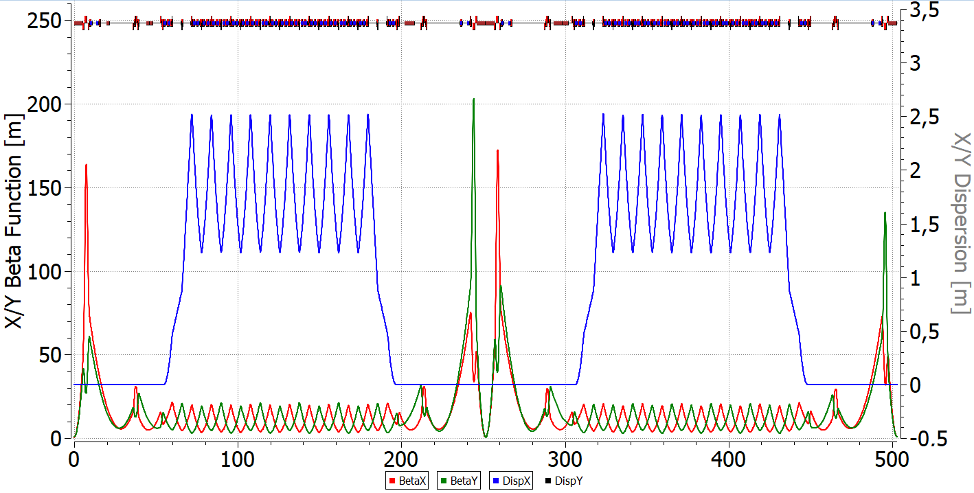
\includegraphics[width=\linewidth]{TEXPaper/img/MOPM071_f2}};
			\end{tikzpicture}
		\end{minipage}
		\hfill
		\begin{minipage}{0.32\linewidth}
			\begin{tikzpicture}
				\node (cone) at (0,0) {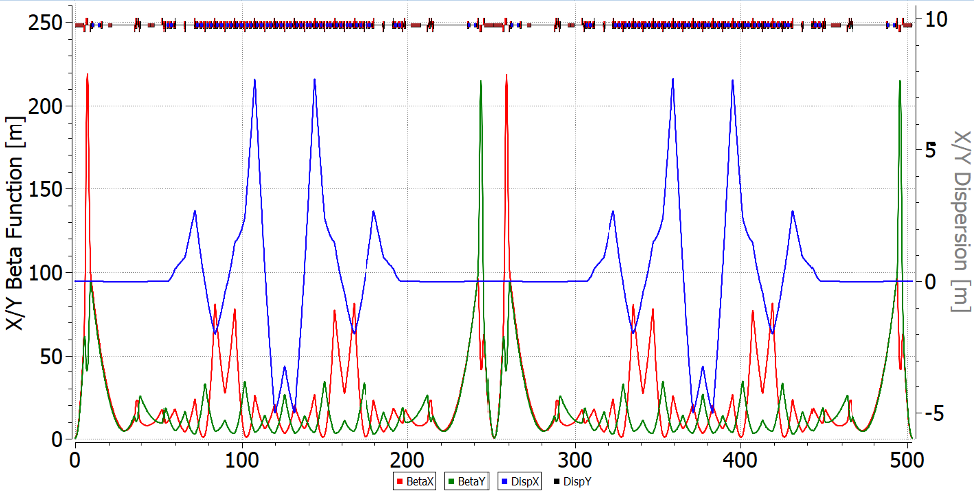
\includegraphics[width=\linewidth]{TEXPaper/img/MOPM071_f1}};
			\end{tikzpicture}
		\end{minipage}
		\begin{minipage}{0.32\linewidth}
			\begin{tikzpicture}
				\node (cone) at (0,0) {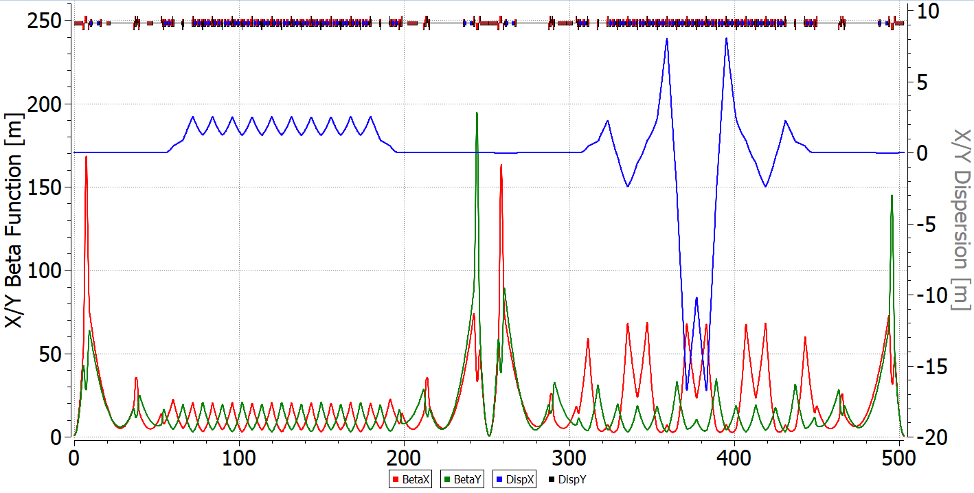
\includegraphics[width=\linewidth]{TEXPaper/img/MOPM071_f3}};
			\end{tikzpicture}
		\end{minipage}
		\newline
}		
\block{STOCHASTIC COOLING}{
		\begin{minipage}{0.32\linewidth}
			\par The cooling rate in the absence of noise [4]
			\begin{equation*}
				\frac{1}{\tau_{\textrm{tr}}}=\frac{W}{N} \frac{\left(1-1 / M_{\textrm{pk}}^2\right)^2}{M_{\textrm{kp}}}
				\label{eq:cooling_rate}
			\end{equation*}
			\noindent The mixing coefficients are defined as
			\begin{equation*}
				\begin{aligned}
					M_{\textrm{pk}} & =\frac{1}{2\left(f_{\max }+f_{\min }\right) \eta_{\textrm{pk}} T_{\textrm{pk}} \frac{\Delta p}{p}}, \\
					M_{\textrm{kp}} & =\frac{1}{2\left(f_{\max }-f_{\min }\right) \eta_{\textrm{kp}} T_{\textrm{kp}} \frac{\Delta p}{p}}
				\end{aligned}
				\label{eq:mixing_coeff}
			\end{equation*}
		\end{minipage}
		\hfill
		\begin{minipage}{0.32\linewidth}
			\par It is evident that asymptotic growth may occur in two scenarios:
			\begin{enumerate}
				\item slip-factor approaches the value $\eta\rightarrow\frac{1}{2\left(f_{\text{max}}+f_{\text{min}}\right)T_{\text{pk}}\delta}$,  Schottky spectrum becomes continuous and $M_{\text{pk}}\rightarrow1$;
				\item slip-factor approaches zero, mixing between the kicker to the pickup does not occur and $M_{\text{kp}}\rightarrow\infty$.
			\end{enumerate}	
		\end{minipage}
		\hfill
		\begin{minipage}{0.32\linewidth}
			\begin{tikzpicture}
				\node (cone) at (0,0) {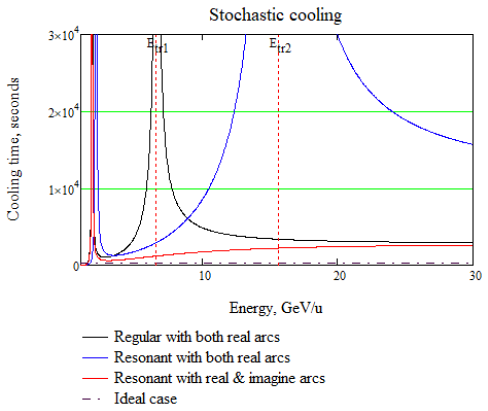
\includegraphics[width=\linewidth]{TEXPaper/img/MOPM071_f4}};
			\end{tikzpicture}
		\end{minipage}
		\newline
}
		
\block{INTRA-BEAM SCATTERING}{

		\begin{minipage}{0.33\linewidth}
			\par Intra-beam scattering represents a fundamental limitation on the beam lifetime in the collider. This is derived from the fundamental principles governing this process [5]
			\begin{equation*}
				\begin{aligned}
					\frac{1}{\tau_{\textrm{IBS}}}=\frac{\sqrt\pi}{4}\frac{cZ^2r_p^2L_C}{A}&\cdot\frac{N}{C_{\mathrm{orb\ }}}\cdot\frac{\left\langle\beta_x\right\rangle}{\beta^3\gamma^3\varepsilon_x^{5/2}\left\langle\sqrt{\beta_x}\right\rangle}\times\\
					&\times\left(\left\langle\frac{D_x^2+{\dot{D}}_x^2}{\beta_x^2}\right\rangle-\frac{1}{\gamma^2}\right)
				\end{aligned}
				\label{eq:ibs}
			\end{equation*}
		 
		\end{minipage}
		\begin{minipage}{0.33\linewidth}
			\par It can be concluded that in a regular lattice, stochastic cooling is able to balance IBS in the energy range $W\geq4.5\ \text{GeV/u}$. To apply stochastic cooling over the entire energy range, the luminosity is sacrificed at low energies by increasing the emittance. In resonant lattices, the IBS time is reduced. For the heavy ions, the configuration should be regular and minimally modulated.
		\end{minipage}
		\hfill
		\begin{minipage}{0.33\linewidth}
			\begin{tikzpicture}
				\node (cone) at (0,0) {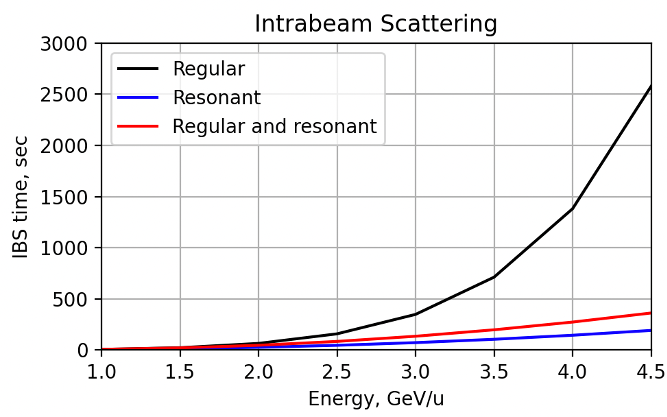
\includegraphics[width=\linewidth]{TEXPaper/img/MOPM071_f5}};
			\end{tikzpicture}
		\end{minipage}
		\newline
}

	\block{REFERENCES}{\hfill	
	\par [1] S.-Y. Lee, {\it Accelerator Physics}, Fourth Edition, World Scientific Publishing Company (Singapore, 2018)
	\par [2] Y.V. Senichev, A.N. Chechenin, Theory of “Resonant” lattices for synchrotrons with negative momentum compaction factor. J. Exp. Theor. Phys. {\bf 105}, 988–997 (2007). doi:10.1134/S1063776107110118
	\par [3] Senichev, Y.V., Chechenin, A.N. Construction of “resonant” magneto-optical lattices with controlled momentum compaction factor. J. Exp. Theor. Phys. {\bf 105}, 1141–1156 (2007). doi:10.1134/S1063776107120060
	\par [4] D. Möhl, G. Petrucci, L. Thorndahl, S. van der Meer, Physics and technique of stochastic cooling. Phys. Rep. {\bf 58}, 75 (1980). doi:10.1016/0370-1573(80)90140-4
	\par [5] 	F. Antoniou, F. Zimmermann, Revision of Intrabeam Scattering with Non-Ultrarelativistic Corrections and Vertical Dispersion for MAD-X. (European Organization for Nuclear Research CERN, 2012), https://cds.cern.ch/record/1445924. Accessed 04 May 2012
	}
	
\end{columns}

\end{document}